% MPE2 simple_world_comm - environment presentation. Build: tectonic presentation/slides.tex
% Figures come from scripts/inspect_env.py, scripts/record.py; the table from scripts/eval_baselines.py.
\documentclass[aspectratio=169,10pt]{beamer}
\usetheme[progressbar=frametitle,numbering=fraction]{metropolis}
\usepackage[polish]{babel}
\usepackage[sfdefault,lining]{FiraSans}
\usepackage{FiraMono}
\usepackage{booktabs}
\usepackage{amsmath}
\usepackage{hyperref}
\graphicspath{{figures/}}

\title{MPE2: Simple World Comm}
\subtitle{Środowisko, agenci losowi, plan pracy}
\author{Jerzy Czarnecki, Mateusz Małachowski}
\institute{Uczenie ze wzmocnieniem}
\date{}

\newcommand{\code}[1]{\texttt{#1}}

\begin{document}

\maketitle

% ---------------------------------------------------------------------------
\begin{frame}{Środowisko i zadanie}
  \begin{columns}[T]
    \begin{column}{0.38\textwidth}
      \centering
      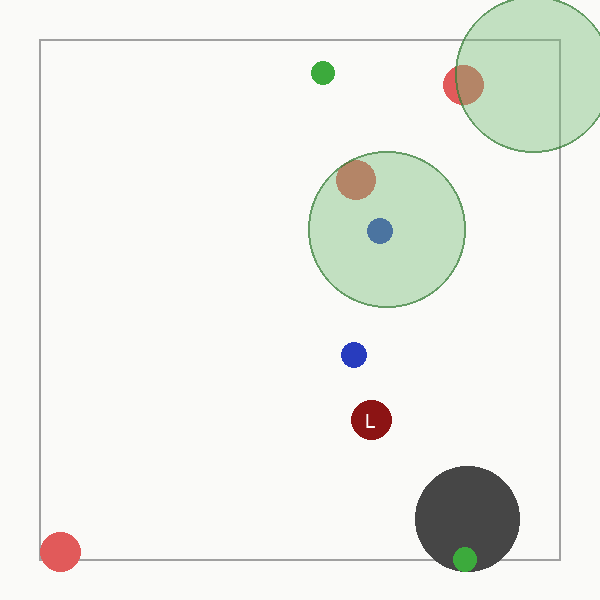
\includegraphics[width=\linewidth]{map_seed0.png}
    \end{column}
    \begin{column}{0.59\textwidth}
      \small
      \begin{itemize}
        \item Ciągła arena 2D, 6 agentów w dwóch drużynach:
          \alert{4 drapieżników} (w tym \alert{lider}) i \alert{2 ofiary}
        \item Na planszy: przeszkoda, 2 jedzenia, 2 lasy
        \item Agent w lesie jest niewidoczny dla agentów spoza tego lasu
        \item Lider widzi wszystkich zawsze i wysyła pozostałym drapieżnikom
          jeden z 4 komunikatów
        \item Ofiary są mniejsze i szybsze (prędkość 1,3 vs 1,0)
        \item Epizod trwa zawsze 25 kroków
      \end{itemize}
      \textbf{Cele}
      \begin{itemize}
        \item drapieżnicy: złapać ofiarę (zderzyć się z nią),
        \item ofiary: uciekać, zbierać jedzenie, nie wychodzić poza arenę.
      \end{itemize}
    \end{column}
  \end{columns}
\end{frame}

% ---------------------------------------------------------------------------
\begin{frame}{Obserwacje i akcje}
  \small
  \centering
  \begin{tabular}{@{}lccc@{}}
    \toprule
    & lider & drapieżnik & ofiara \\
    \midrule
    obserwacja & \code{Box(34)} & \code{Box(34)} & \code{Box(28)} \\
    akcje & \code{Discrete(20)} & \code{Discrete(5)} & \code{Discrete(5)} \\
    \bottomrule
  \end{tabular}\\[8pt]
  \raggedright
  \textbf{Obserwacja} (wektor liczb, względem agenta)
  \begin{itemize}
    \item własna prędkość i pozycja
    \item względne pozycje przeszkody, jedzenia i lasów oraz pozostałych agentów
      (\code{(0,0)}, gdy agent jest ukryty w lesie)
    \item prędkości ofiar, czy agent jest w lesie; drapieżnicy dostają też komunikat lidera
  \end{itemize}
  \textbf{Akcje}
  \begin{itemize}
    \item ruch: stój, lewo, prawo, dół, góra
    \item lider: 4 komunikaty $\times$ 5 ruchów $=$ 20 akcji
  \end{itemize}
  Stan globalny (\code{state()}, 192 liczby) = połączone obserwacje wszystkich agentów
\end{frame}

% ---------------------------------------------------------------------------
\begin{frame}{Funkcja nagrody i koniec epizodu}
  \small
  \textbf{Drapieżnicy} (nagroda wspólna dla drużyny + kształtowanie):
  \[
    r_{\text{drap}} = 5 \cdot \#\text{zderzeń drapieżnik--ofiara} \;-\; 0{,}1 \cdot d(\text{najbliższa ofiara})
  \]
  \textbf{Ofiary} (nagroda indywidualna):
  \[
    r_{\text{ofiara}} = -5 \cdot \#\text{zderzeń z drapieżnikiem} + 2 \cdot \#\text{jedzenia}
    - 0{,}05 \cdot d(\text{najbliższe jedzenie}) - 2 \sum_{\text{osie}} \text{kara}(|x|)
  \]
  kara za wyjście z areny: 0 dla $|x| < 0{,}9$, rośnie do 10 poza $|x| > 1$
  \begin{itemize}
    \item \textbf{Koniec epizodu}: zawsze po 25 krokach (\code{truncated})
  \end{itemize}
  \textbf{Trudności}
  \begin{itemize}
    \item rywalizacja: przeciwna drużyna też się uczy, więc środowisko zmienia się w trakcie treningu,
    \item lasy ukrywają agentów, czyli obserwacje są częściowe,
    \item komunikaty lidera na starcie nic nie znaczą; ich sens drużyna musi wypracować,
    \item wspólna nagroda drapieżników: trudno ocenić wkład pojedynczego agenta.
  \end{itemize}
\end{frame}

% ---------------------------------------------------------------------------
\begin{frame}{Możliwości konfiguracji}
  \begin{columns}[T]
    \begin{column}{0.66\textwidth}
      \small
      \textbf{Parametry} \code{simple\_world\_comm\_v3.parallel\_env(...)}
      \begin{itemize}
        \item \code{num\_good} (2), \code{num\_adversaries} (4): liczebność drużyn
        \item \code{num\_obstacles} (1), \code{num\_food} (2), \code{num\_forests} (2)
        \item \code{max\_cycles} (25): długość epizodu
        \item \code{continuous\_actions} (False): akcje dyskretne lub ciągłe
      \end{itemize}
      \textbf{API}
      \begin{itemize}
        \item PettingZoo: tryb równoległy (wszyscy agenci działają naraz) lub turowy (AEC)
        \item seed: losowe pozycje agentów, jedzenia, lasów i przeszkody
      \end{itemize}
    \end{column}
    \begin{column}{0.30\textwidth}
      \centering
      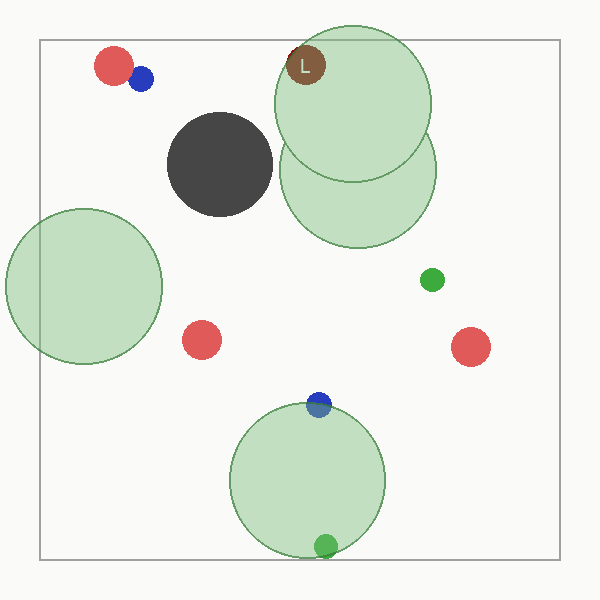
\includegraphics[height=0.37\textheight]{forests_4.png}\\[6pt]
      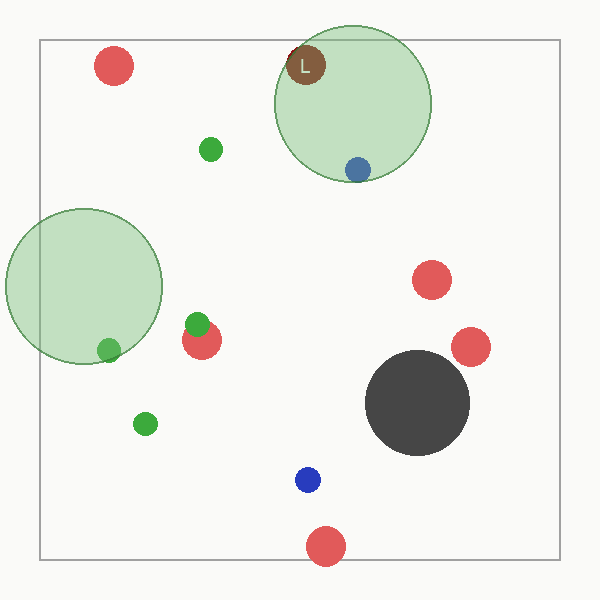
\includegraphics[height=0.37\textheight]{agents_6v4.png}
    \end{column}
  \end{columns}
\end{frame}

% ---------------------------------------------------------------------------
\begin{frame}{Agenci losowi}
  \centering
  % the strip links to the video; the mp4 is played separately during the talk
  \href{run:media/random_agents.mp4}{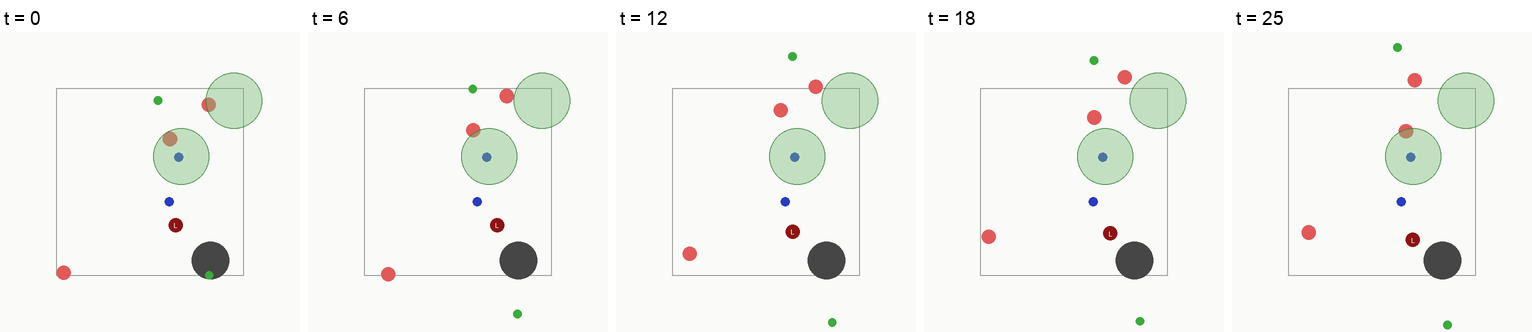
\includegraphics[width=\textwidth]{random_strip.png}}
\end{frame}

% ---------------------------------------------------------------------------
\begin{frame}{Agenci losowi i heurystyczni: wyniki (1000 epizodów)}
  \centering
  \scriptsize
  % generated by scripts/eval_baselines.py - do not edit
\begin{tabular}{@{}llrrrrr@{}}
\toprule
drapieżnicy & ofiary & nagroda drap. & nagroda ofiar & złapania & epiz. ze złapaniem & ofiary poza areną \\
\midrule
losowi & losowi & 3,4 & -23,8 & 1,12 & 40\% & 20\% \\
heurystyczni & losowi & 34,4 & -41,1 & 6,69 & 98\% & 21\% \\
losowi & heurystyczni & 3,0 & -2,7 & 1,03 & 41\% & 2\% \\
heurystyczni & heurystyczni & 18,1 & -11,9 & 3,71 & 91\% & 3\% \\
\bottomrule
\end{tabular}
\\[4pt]
  \raggedright
  \small
  \textbf{Heurystyka}: drapieżnicy gonią najbliższą widoczną ofiarę; ofiary idą do jedzenia,
  odsuwają się od bliskich drapieżników i pilnują areny
  \begin{itemize}
    \item losowe ofiary tracą głównie przez wychodzenie poza arenę (20\% kroków)
    \item losowi drapieżnicy łapią ofiarę przypadkiem w 39\% epizodów, heurystyczni w 90--97\%
    \item lasy prawie nie zmieniają wyników tych polityk (90\% złapań przy 2 lasach, 93\% bez lasów)
  \end{itemize}
\end{frame}

% ---------------------------------------------------------------------------
\begin{frame}{Plan dalszej pracy}
  \begin{itemize}
    \setlength{\itemsep}{12pt}
    \item \textbf{Algorytm}: MAPPO; każda drużyna ma własnych aktorów
      i krytyka widzącego stan globalny
    \item \textbf{Cel pośredni}: drapieżnicy MAPPO lepsi od heurystycznych przeciwko heurystycznym ofiarom
      i odwrotnie
    \item \textbf{Cel końcowy}: obie drużyny trenowane jednocześnie; każda lepsza od baseline'ów
  \end{itemize}
\end{frame}

% ---------------------------------------------------------------------------
\begin{frame}{Baseline i metryki}
  \textbf{Baseline}
  \begin{itemize}\small
    \item drużyny losowe i heurystyczne (poprzedni slajd)
    \item w literaturze brak opublikowanych wyników dla tego środowiska; pochodzi ono z filmu
      do pracy o MADDPG [1]; MAPPO osiąga dobre wyniki na kooperacyjnych zadaniach MPE [2]
  \end{itemize}
  \textbf{Metryki}
  \begin{itemize}\small
    \item średnia nagroda każdej drużyny
    \item złapania: liczba, odsetek epizodów ze złapaniem, krok pierwszego złapania
    \item ofiary: czas przy jedzeniu, czas poza areną, czas w lesie
    \item komunikacja: czy lider używa różnych komunikatów (entropia)
    \item ocena przeciwko stałym przeciwnikom (losowym, heurystycznym) i krzywe uczenia z kilku seedów
  \end{itemize}
  \vfill
  {\tiny
    [1] R. Lowe i in., \emph{Multi-Agent Actor-Critic for Mixed Cooperative-Competitive Environments}, NeurIPS 2017\par
    [2] C. Yu i in., \emph{The Surprising Effectiveness of PPO in Cooperative Multi-Agent Games}, NeurIPS 2022\par}
\end{frame}

\end{document}
